\subsection{Regional polarization}

The geography of mobility has received considerable attention over the past few years,\footnote{See \cite{Chetty2014Land} and \cite{Bell2018Land} amongst others.} and in this section we turn to exploring the regional dimension of our data. We focus on two aspects, both of which address the hypothesis that the observed increase in the impact of parental income on occupational outcomes is related to the polarization of employment. The next subsection considers whether the reduction in mobility that we have identified appears when we replace the cohort dummies by a measure of the extent of polarization that individuals faced in their region when they were young. It hence asks if the cohort dummies are capturing the differences in the structure of the labour market over time. Our second strategy consists in estimating the impact of parental income on occupational outcomes at the regional level in order to get regional measures of mobility. We then ask whether there is a correlation between the changes over time in regional mobility and the increase in polarization at the local level.

Our data have information on 10 regions and hence do not allow us to identity the very local effects that other work has observed.\footnote{\cite{Chetty2014Land} focus on considerably smaller locations in their analysis for the US. For the UK, \cite{Bell2018Land} consider a dataset with the 32 NUTS2 regions but which does not have information on parental income.} For both analyses we need to construct a measure of polarization at the regional level, but we are impaired by the fact that sample sizes at the regional level are small and thus measures of regional polarization based on our cohort data may not capture well the actual changes in the structure of employment. In order to have a more representative sample we use data from the Labour Force Survey (LFS) to build polarization measures. 

When computing the extent of polarization we face two concerns. First, as shown in the appendix, the share of middling employment has fallen in all regions, but whether this has occurred at the expense of low-paying or high-paying occupations varies. For this reason, rather than focusing exclusively on the share of middling jobs we consider changes in the share of jobs in all three occupations. Second, we need to define the job market that individuals in our dataset were facing and measure the extent of polarization in that particular market. To do so we consider the distribution of employment for the relevant age cohorts in the LFS. We hence suppose that members of a cohort are in competition for jobs with individuals that were born in the 5 years before and 5 years after them. That is, for the NCDS58 cohort we consider individuals born between 1953 and 1963, and for the BCS70 those born between 1965 and 1975. We measure the share of employment in each year between the initial and final period that we use for each cohort, and compute the average over the whole period in which each cohort has been exposed to employment changes. That is, for the NCD58 we consider the structure of employment between 1981 and 2000, for the BCS70 between 1996 and 2012. We then measure the extent of polarization as changes in the occupational shares obtained for the 1953-63 cohorts and those for the 1965-75 ones. Appendix \ref{chap2-app-data-LFS} gives details on the LFS data and our measures of polarization, and shows that all regions exhibited an increase in polarization (see Figure \ref{chap2-fig:lfs-change}).


\subsection{Individual outcomes and regional employment patterns}

Several factors may be behind the increased importance of parental income for occupational outcomes across cohorts. Here we explore the possibility that employment polarization is one of these factors. To do so, we substitute the cohort dummy used in our regressions by our measure of regional polarization. We use the region in which the individual lived at age 16, and measure polarization in that region as the share of middling employment in the year in which the individuals are 23/26.

Table \ref{chap2-tab:regocc-multi2A-short} displays the results obtained from the multinomial regression, regression, with the first three columns reporting again the estimates when we use the cohort dummies (i.e. those in Table \ref{chap2-tab:occ-multi2-short} above), and the last three columns those in which we substitute the dummies for the share of non-middling jobs and this share interacted with parental income (both standardized). The regressions also include a region fixed effect. We focus on the effect of the share of non-middling employment as an increase in its value can be interpreted as an increase in polarization. \footnote{Results using jointly the low- and high-paying employment shares are reported in Table \ref{chap2-tab:regocc-multi2B-short} in the appendix. We also used alternative measures of polarization using data on only the initial year measure of polarization for each cohort (1981 and 1996) rather than the average over the working-life and found equivalent results to those reported here (results not reported).} 
\begin{table}[!tb]
    \centering
    \caption{Second-period occupation probability according to share of non-middling occupations in the region at the age 16}
    \label{chap2-tab:regocc-multi2A-short}
    \resizebox*{\textwidth}{!}{
    \begin{threeparttable}
        \setlength{\tabcolsep}{0pt}
        \begin{tabular}{l D{.}{.}{5.3} D{.}{.}{5.5} D{.}{.}{5.5} D{.}{.}{5.3} D{.}{.}{5.5} D{.}{.}{5.5}}
\toprule
 & \multicolumn{6}{c}{Multinomial logit - Dep. var.: Second-period occupation} \\
\cmidrule(lr){2-7}
 & \multicolumn{3}{c}{(1)} & \multicolumn{3}{c}{(2)} \\
\cmidrule(lr){2-4}\cmidrule(lr){5-7}
 & \multicolumn{1}{c}{Low} & \multicolumn{1}{c}{Mid} & \multicolumn{1}{c}{High} & \multicolumn{1}{c}{Low} & \multicolumn{1}{c}{Mid} & \multicolumn{1}{c}{High} \\
\midrule
BCS cohort                        & 0.05   & -0.03      & 0.11       &        &            &            \\
                                  & (0.11) & (0.09)     & (0.09)     &        &            &            \\
Non-Middling share                &        &            &            & 0.07   & 0.02       & 0.17^{***} \\
                                  &        &            &            & (0.06) & (0.05)     & (0.05)     \\
Parental income                   & 0.01   & 0.04       & 0.19^{***} & 0.04   & 0.11^{***} & 0.35^{***} \\
                                  & (0.04) & (0.04)     & (0.04)     & (0.03) & (0.03)     & (0.03)     \\
Par. inc. $\times$ BCS            & 0.05   & 0.16^{***} & 0.36^{***} &        &            &            \\
                                  & (0.06) & (0.05)     & (0.05)     &        &            &            \\
Par. inc. $\times$ Non-Mid. share &        &            &            & -0.00  & 0.04^{*}   & 0.11^{***} \\
                                  &        &            &            & (0.03) & (0.02)     & (0.02)     \\
\midrule
Num. obs. & \multicolumn{1}{c}{14763} & \multicolumn{1}{c}{14763} & \multicolumn{1}{c}{14763} & \multicolumn{1}{c}{14763} & \multicolumn{1}{c}{14763} & \multicolumn{1}{c}{14763}\\
\bottomrule
\end{tabular}

        \begin{tablenotes}[flushleft]
            \footnotesize{\item\textit{Notes}: 
            % Stars and SE
            $^{***}p<0.01$; $^{**}p<0.05$; $^{*}p<0.1$. Standard errors between parentheses. 
            % Baseline outcome
            Out-of-work occupation in second period is the base outcome of the multinomial logistic regression.
            % Referent group
            Male in the NCDS58 cohort is the referent group in (1), while male is the referent group in (2).
            % Variables details
            Parental income in logarithm and then standardized at the cohort level. 
            Non-middling share corresponds to the share of occupations that are not middling, hence, low-paying and high-paying, in total employment in the region at age 16. The shares has been standardized for the interpretability of coefficients when interacted with parental income.
            % Control variables
            Control variables in (1) include Intercept, Female and Female $\times$ BCS, while control variables in (2) include Intercept, Female and Female $\times$ Non-Mid. share. %; see Table \ref{chap2-tab:tobefilled} in the appendix for these coefficients.
            }
        \end{tablenotes}
    \end{threeparttable}
    }
\end{table}

The coefficients of interest have the expected sign. A higher share of non-middling employment is associated with a greater average probability of being in a high-paying occupation, as we would expect given the greater availability of these jobs. There is no significant effect on the other employment categories, implying that higher polarization does not affect the allocation of workers between out-of-work, low-paying jobs and middling jobs. Parental income has, as expected, a positive impact on the likelihood to be in middling and high-paying jobs, and the interaction terms indicate that as polarization increases the effect of background becomes stronger. To gauge the magnitude of these effects, we average the (standardized) share of middling employment across regions for each cohort, obtaining that for the NCDS58 (resp. BCS70) it is 0.845 standard deviations below (above) the mean. Using these figures, the coefficients on column (6) imply that a one standard deviation increase in parental income raised the probability of being in a high-paying occupation by 0.14 pp. for the older cohort and by 0.44 for the younger one. These values are close to those obtained in our core specification (column (3)) of 0.19 and 0.55, indicating that using the differences in polarization across cohorts yield effects that are close to those obtained with the cohort dummy. 


\subsection{Regional mobility} 

Our final step consists in exploiting the cross-sectional variation in the regional data to consider the correlation between regional mobility and polarization. We start by running the same multinomial regressions as in equation \ref{chap2-eq:emp-multi3} but at the regional level.\footnote{We do not compute first-period mobility and conditional second-period mobility because of sample sizes, as in many regions we have only a small number of individuals moving across certain occupations between first and second period.} Table \ref{chap2-tab:reg-multi2-short} presents the coefficients on parental income obtained when we regress second period occupation on parental income. As before, we need to recall that these are the coefficients relative to the probability of being out-of-work (see also Figures \ref{chap2-fig:reg-multi2-pinc-male} and \ref{chap2-fig:reg-multi2-pinc-female} in the appendix).

\begin{table}[!tb]
    \centering
    \caption{Probability of second-period occupation by region}
    \label{chap2-tab:reg-multi2-short}
    \resizebox*{!}{\dimexpr\textheight-2\baselineskip\relax}{
    \begin{threeparttable}
        \centering
        \setlength{\tabcolsep}{12pt}
        \begin{tabular}{l D{.}{.}{3.5} D{.}{.}{3.5} D{.}{.}{3.5}}
\toprule
 & \multicolumn{3}{c}{Multi. logit - Dep. var.: Second-period occupation} \\
\cmidrule(lr){2-4}
 & \multicolumn{1}{c}{Low-paying} & \multicolumn{1}{c}{Middling} & \multicolumn{1}{c}{High-paying} \\
\midrule
\midrule
 East Anglia (N = 904) & & & \\
\midrule
Par. inc.              & 0.04       & -0.00       & 0.13        \\
                       & (0.15)     & (0.14)      & (0.14)      \\
Par. inc. $\times$ BCS & -0.10      & 0.31        & 0.57^{**}   \\
                       & (0.25)     & (0.26)      & (0.26)      \\
\midrule
 East Midlands (N = 1066) & & & \\
\midrule
Par. inc.              & 0.06       & 0.12        & 0.17        \\
                       & (0.15)     & (0.15)      & (0.15)      \\
Par. inc. $\times$ BCS & 0.45^{**}  & 0.44^{**}   & 0.92^{***}  \\
                       & (0.22)     & (0.21)      & (0.21)      \\
\midrule
 North (N = 1037) & & & \\
\midrule
Par. inc.              & -0.04  & -0.08       & 0.02        \\
                       & (0.15) & (0.14)      & (0.14)      \\
Par. inc. $\times$ BCS & 0.07   & 0.34        & 0.58^{***}  \\
                       & (0.22) & (0.22)      & (0.21)      \\
\midrule
 North West (N = 1810) & & & \\
\midrule
Par. inc.              & 0.12       & 0.06        & 0.32^{***}  \\
                       & (0.11)     & (0.10)      & (0.11)      \\
Par. inc. $\times$ BCS & -0.01      & 0.32^{**}   & 0.35^{**}   \\
                       & (0.16)     & (0.15)      & (0.15)      \\
\midrule
 Scotland (N = 1489) & & & \\
\midrule
Par. inc.              & 0.03   & 0.13        & 0.14        \\
                       & (0.12) & (0.12)      & (0.12)      \\
Par. inc. $\times$ BCS & 0.18   & 0.17        & 0.52^{***}  \\
                       & (0.18) & (0.18)      & (0.17)      \\
\midrule
 South East (N = 3718) & & & \\
\midrule
Par. inc.              & 0.01       & 0.06        & 0.17^{**}   \\
                       & (0.09)     & (0.08)      & (0.08)      \\
Par. inc. $\times$ BCS & -0.06      & 0.02        & 0.26^{**}   \\
                       & (0.11)     & (0.11)      & (0.11)      \\
\midrule
 South West (N = 1141) & & & \\
\midrule
Par. inc.              & -0.10      & 0.05        & 0.17        \\
                       & (0.16)     & (0.16)      & (0.16)      \\
Par. inc. $\times$ BCS & 0.08       & -0.02       & 0.31        \\
                       & (0.21)     & (0.21)      & (0.21)      \\
\midrule
 Wales (N = 821) & & & \\
\midrule
Par. inc.              & -0.23  & -0.16       & -0.07      \\
                       & (0.17) & (0.16)      & (0.16)     \\
Par. inc. $\times$ BCS & 0.34   & 0.27        & 0.62^{***} \\
                       & (0.24) & (0.23)      & (0.22)     \\
\midrule
 West Midlands (N = 1495) & & & \\
\midrule
Par. inc.              & 0.04   & 0.12        & 0.63^{***}  \\
                       & (0.12) & (0.12)      & (0.14)      \\
Par. inc. $\times$ BCS & 0.09   & 0.12        & -0.08       \\
                       & (0.17) & (0.17)      & (0.18)      \\
\midrule
 Yorkshire and Humberside (N = 1282) & & & \\
\midrule
Par. inc.              & 0.03   & -0.05       & 0.02        \\
                       & (0.14) & (0.12)      & (0.12)      \\
Par. inc. $\times$ BCS & 0.06   & 0.21        & 0.53^{***}  \\
                       & (0.19) & (0.17)      & (0.17)      \\
\bottomrule
\end{tabular}

        \begin{tablenotes}[flushleft]
            \footnotesize{\item \textit{Notes}: 
            % Stars and SE
            $^{***}p<0.01$; $^{**}p<0.05$; $^{*}p<0.1$. Standard errors between parentheses. 
            % Baseline outcome
            Out-of-work occupation in second period is the base outcome of the multinomial logistic regression.
            % Referent group
            Male in the NCDS58 cohort is the referent group.
            % Variables details
            Parental income in logarithm and then standardized at the cohort level.
            % Control variables
            Control variables in all regressions include Intercept, BCS cohort, Female and Female $\times$ BCS.}
        \end{tablenotes}
    \end{threeparttable}
    }
\end{table}

These regressions allow us to make two inferences. First, we can ask whether the changes in occupational mobility observed across cohorts at the national level also took place at the regional level and are not the result of the population reallocating across regions with different mobility patterns. When we split the data we find that for the vast majority of regions (7/10) parental income exhibits insignificant coefficients for the older cohort. Only in the North West, the South East and the West Midlands do we find a significant coefficient on parental income. Note, however, that out of the seven regions for which the coefficient is not significant, 4 of them have magnitudes close to the 0.19 point estimate we obtained at the national level. The lack of significance can then be due to a lack of statistical power given the limited number of observations (per region and also in certain region-occupation cells). For those born in 1970, the likelihood to be in a high-paying occupation exhibits systematically large and significant coefficients on parental income. Out of the 10 regions only two (South West and West Midlands) do not display a significant coefficient. In all the others, the magnitude of the effect is large, with the coefficient being at least twice as large for the younger as for the older cohort (eg. North West) and much larger in others. These results indicate that the increase in the importance of parental income across cohorts holds at the regional level.

Second, the estimates imply large variations in the degree of inter-generational income mobility across locations, with the probability of someone born in a household in the bottom quintile moving to the top quintile being three times higher in the most than in the least mobile locations. This raises the question of whether the magnitude of the changes in mobility is correlated to the degree of employment polarization observed at the regional level. 

To capture changes in mobility in region $r$, we consider the between-cohort change in the role of parental income for being in a high-paying occupation, namely, $\Delta\beta_H^r$. These coefficients correspond to the ``$\text{Par. Inc. }\times\text{ BCS}$'' coefficients in Table \ref{chap2-tab:reg-multi2-short}. The change in the extent of regional polarization is measured by the change across cohorts in regional polarization as measured from the LFS. Figure \ref{chap2-fig:regocc-absolute-high} displays the correlation between the two variables, with both measured in percentage points. The three panels report, in the horizontal axis, the changes in absolute value of the share of employment in each of the three categories. The actual changes are positive for high- and low-paying occupations and negative for middling ones, hence reporting the absolute value implies that for all three occupational categories moving from the left to the right of each graph implies an increase in polarization. The vertical axis displays the regional $\Delta\beta_{H}$ described above.
\begin{figure}[!tb]
    \centering
    \caption{Change in parental income coefficient for high-paying second-period occupation according to job polarization at the regional level}
    \label{chap2-fig:regocc-absolute-high}
    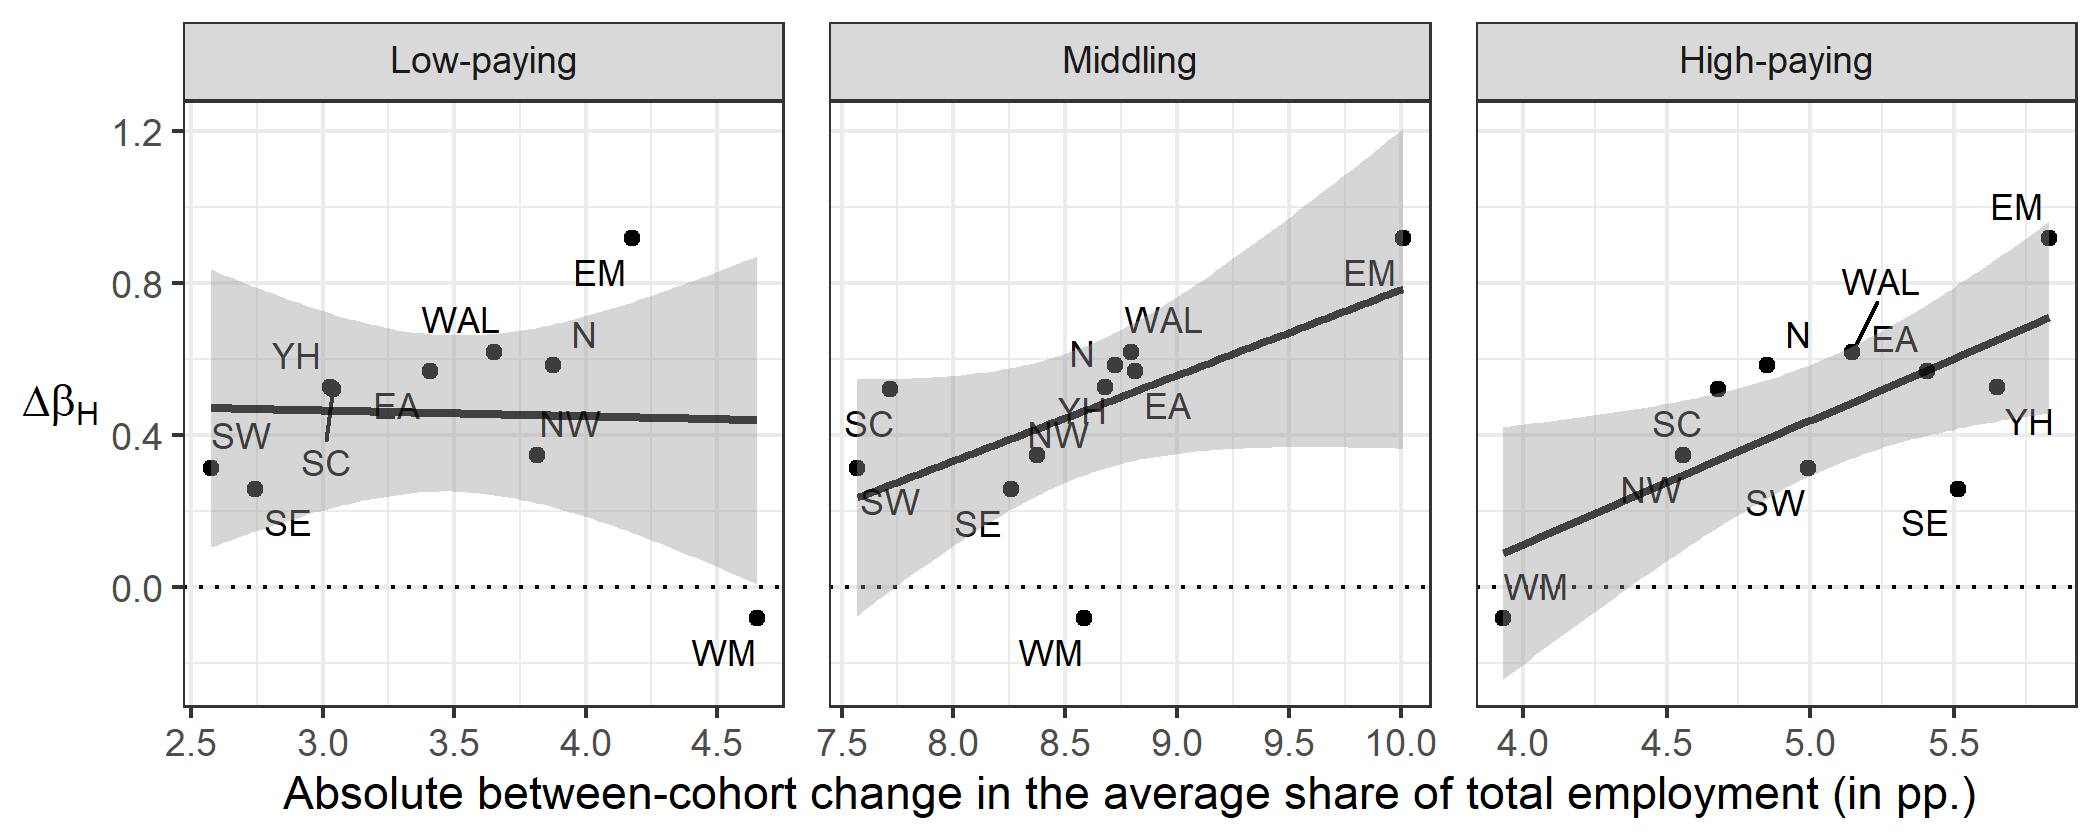
\includegraphics[width=\linewidth]{chap2/graphic/regocc-absolute-high.png}
    \vspace{-3em}
	\justify\singlespacing\footnotesize{\textit{Notes:} This figure presents the correlation across regions between the change in the parental income coefficient for the high-paying occupation in second period $\Delta\beta_H$ and the between-cohort change in absolute value in the average share of total employment of low-paying, middling, and high-paying occupations, in percentage points. Note that, by taking the absolute value of the change, we reversed the x-axis for the middling panels (middle column). Thus, regions on the left-hand (resp. right-hand) side of each panel are those where the polarization of employment has been lower (resp. larger).}
\end{figure}

Each dot represents one of the 10 regions, while the line corresponds to the linear regression line.\footnote{Figure \ref{chap2-fig:regocc-absolute-all} in the appendix presents equivalent graphs for the change in the coefficients on parental income in the probability of being in middling and low-paying occupations, namely, $\Delta\beta_{M}$ and $\Delta\beta_{L}$. We obtain broadly similar results in the two cases,} Consider the right-most graph. The upward slope indicates that regions where the share of high-paying occupations (in the relevant age group) increased the most are also the regions where the impact of parental income in accessing high-paying occupations rose the most. Similarly, the middle graph also displays an upwards-slopping schedule when we plot the magnitude of the change in the share of middling occupations against $\Delta\beta_{H}$, indicating that regions where the share of middling income jobs declined the most are also those where parental impact became strongest. The left-hand graph depicts the correlation between the change in the coefficient and the change in the share of low-paying occupations, and displays a flat schedule, which is driven by an outlier, the West-Midlands. Removing this observation, yields a positive correlation between the change in polarization and the change in the effect of parental income.

This subsection, together with the previous one, provide suggestive evidence that the increase in employment polarization may be a cause of the reduction in occupational mobility observed across the two cohorts. When we exploit the time dimension, we find that differences in the extent of polarization experienced by the two cohorts result in estimates of the impact of parental income that are close to those obtained when using cohort dummies. The cross-sectional evidence, in turn, indicates that when we estimate mobility measures by regions, the increases in \emph{immobility} that we observe are correlated with regional increases in polarization.




